\section{Introduction} \label{sec:introduction}

Agent-Based Model Simulation (ABMS) addresses problems in basic science and applied sectors ranging from infrastructure to public health to
telecommunications.
Although the aplication domains are varied, there is a common theme of interest in cross-scale dynamics.
However, to fully realize this potential, ABMS require sufficient scale to capture the systems' emergent behaviors.
Advances in HPC have greatly increased the power of ABMS to andwer scientific questions, and the advent of fabric-based accelerator architectures such as the Cerebras Wafer Scale Engine (WSE) have the potential to do a huge jump of capability.

\subsection{Agent-based Evolution Simulation}

Within the domain of ABMS, evolutionary modeling is one thing.
artificial life (open-ended evolution) and evolutionary epidemiology, ecology, AND blah as well as scenarios where replicating entities like cultural artifacts or computer viruses.
Evolutionary questions often explicitly span scopes.
Not only individual populations, but rich ecologies of interacting populations and multicellular organisms \citep{morenoDISHTINYTODO}.
Unlike other types of simulation, evolutionary simulation can often tolerate great deals of flexible asynchronicity and local structure.
The ability to have flexible, entirely independent execution within processor elements is important too because the underlying computation is highly heterogeneous with a cell and changes over evolutionary time.
At the frontiers of evolutionary computation, there is in particular growing interest in the question of ``open-ended evolution'' \citep{alifeworkshopsTODO}.
This refers to the problem of the inability to recreate the ongoing generation of novelty, complexity, and adaptation within the natural world.
To this end, paradigm-changing advances in massively-distributed, spatial computing being highlighted as of particular interest \citep{ackleyTODO}.

% TODO cite DOE working paper from EXPRESS grant
Emerging class of fabric-based architectures epitomized by the Cerebras Wafer Scale Engine have great promise to advance ABM \citep{lauterbach2021path,lie2022cerebras}.
This class of technologies unifies hundreds of thousands of computational elements embeded in memory with a spatial interconnect.
but the field of evolutionary computation is a particularly good thematic and algorithmic fit and, indeed, has established interest and open calls for this type of scale-up but it has yet to be acted upon.
The unique capabilities of the CS-2 platform will allow us to push the boundaries of model-based inquiry, allowing investigation of new questions at the magnitude of continental or global-scale population structure and at the resolution of individual-level immunological responses.
To run massive models necessary to test our ``best effort" observability approaches, we will target the 850,000 core Cerebras Wafer Scale Engine, which features a fabric architecture epitomic of emerging accelerator memory and I/O challenges; however, our proposed methodology generalizes to other domains and HPC hardware systems.

As the hardware has become available, methodological limitations have been holding back its potential within this field.
Our goal for this project is to lay the groundwark for harnessing this cutting-edge hardware --- and positioning the field to continue to benefit from this emerging class of hardware accelerators.
Reaching these goals, needs methodological development .
In particular, need to be able to observe a simulation for it to be scientifically useful.

Phylogenetic history is an important part of that (steal citations from arxiv papers)

A particular focus of our work is in the design of new algorithms to improve the observability of agent-based evolutionary simulations at scale through extraction of agent (e.g., pathogen) phylogenetic histories.
This information is known to provide insight into underlying evolutionary/epidemiological dynamics within a system.
Further, comparison of observed phylogenies against simulation phylogenies can be used to evaluate hypotheses for underlying dynamics within real-life evolutionary/epidemiological systems.

% https://github.com/mmore500/phylotrack-algorithm-analysis/blob/fe16d2b2d7df99faade09c01b72f681160749f51/tex/text/body/introduction.tex
In addition to addressing questions of natural history, access to the phylogenetic record of biological life has proven informative to conservation biology, epidemiology, medicine, and biochemistry among other domains \citep{faithConservationEvaluationPhylogenetic1992, STAMATAKIS2005phylogenetics, frenchHostPhylogenyShapes2023,kim2006discovery}.
Nonetheless, existing analyses of phylogenetic structure within digital systems have already proven valuable, enabling diagnosis of underlying evolutionary dynamics \citep{moreno2023toward,hernandez2022can,shahbandegan2022untangling, lewinsohnStatedependentEvolutionaryModels2023a} and even serving as mechanism to guide evolution in application-oriented domains \citep{lalejini2024phylogeny,lalejini2024runtime,murphy2008simple,burke2003increased}.

Further, comparison of observed phylogenies against simulation phylogenies can be used to evaluate hypotheses for underlying dynamics within real-life evolutionary/epidemiological systems \citep{TODOtheGenevaHIVpaper}.

\subsection{Phylogenetic Tracking Methods}

Historically, simulation phylogenies have typically only been collected using a centralized, complete record-keeping approach suited to serial simulation.
Substantial limitations and costs to scaling this up \citep{morenoTODOpreprint}.

\begin{figure}[htbp]
\centering
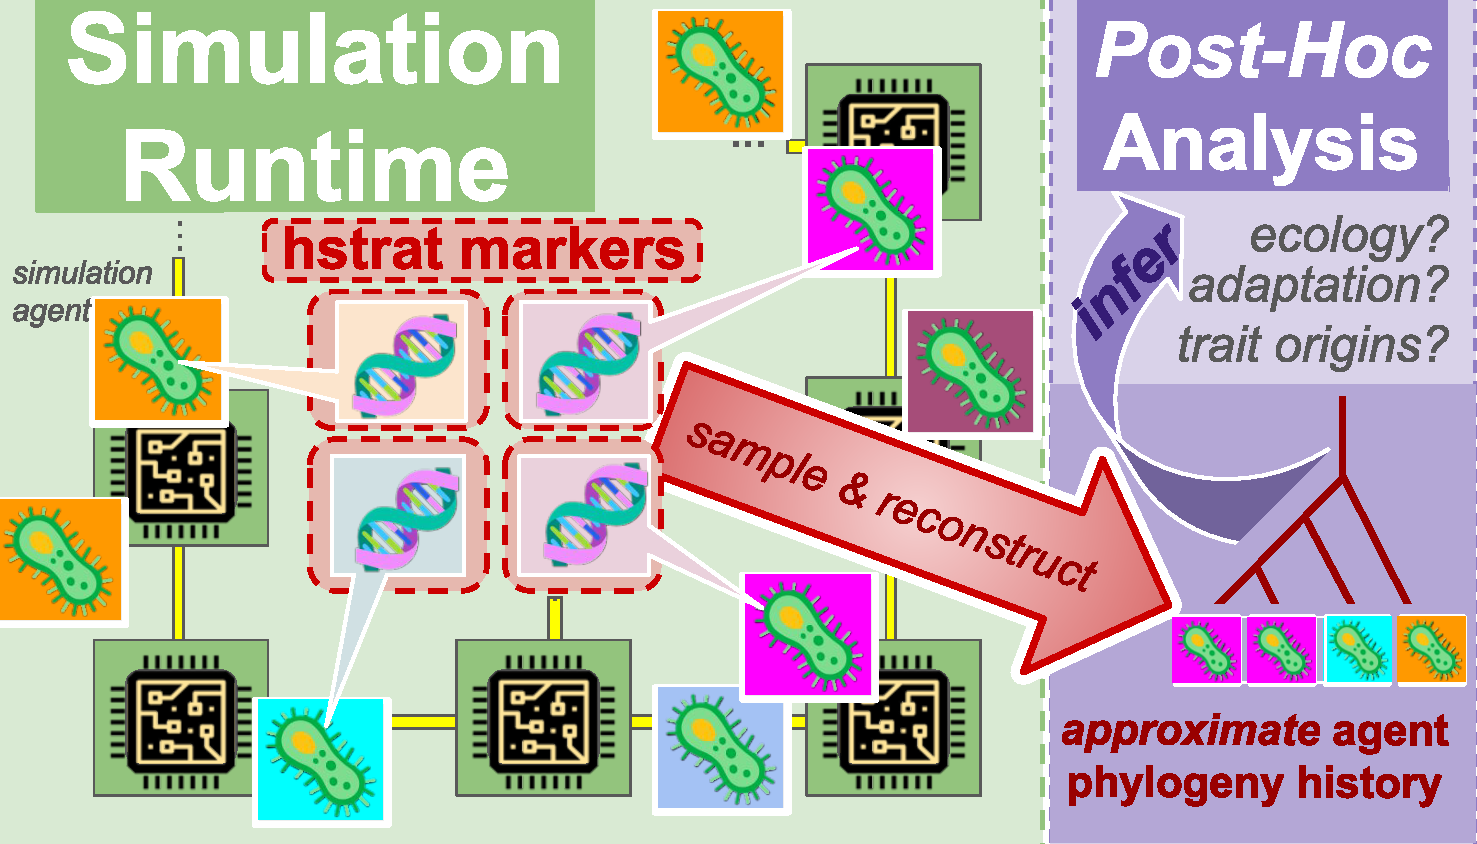
\includegraphics[width=4in]{img/runtime-posthoc-schematic.pdf}
\caption{Proposed agent-based evolutionary simulation and observation framework, using HStrat markers to estimate phylogenetic history, thereby, infer evolutionary dynamics.}
\label{fig:runtime-posthoc-schematic}
\end{figure}

To overcome this limitation, we have proposed a new class of reconstruction-based approaches to phylogenetic tracking in silico \citep{moreno2022hereditary}.
These approaches require no data collection during simulation runtime; instead, they use post hoc comparisons between end-state agents to deduce approximate phylogenetic history (Figure \ref{fig:runtime-posthoc-schematic}).
Although reconstruction biological genomes takes gobs of data, because genetic components in digital evolution can be explicitly designed we have been able to achieve high quality reconstructions with on the order of 96 bits of overhead per agent.
Early evaluations of this revised approach have achieved high-quality reconstruction of phylogenetic histories for tens of thousands of fully-distributed agents using just 96 bits of tracking information per agent.
Details on this is provided in Section \ref{sec:methods}.
